\documentclass[a4paper,12pt]{article}
\usepackage{graphicx, geometry, subfigure, amsmath, adjustbox, array}
\usepackage{xcolor}
\geometry{a4paper,left=2cm,right=2cm,top=1cm,bottom=2cm}
\setlength{\baselineskip}{12pt}
\renewcommand\arraystretch{1.5}
\renewcommand{\d}{\mathrm{d}}
\newcommand{\cm}{\mathrm{cm}}
\newcommand{\s}{\mathrm{s}}
\newcommand{\g}{\mathrm{g}}

\title{\textbf{Stars and Planets Problem Set3}}
\author{Qingru Hu}
\date{\today}

\begin{document}
\maketitle
\section*{\textbf{Exercise \uppercase\expandafter{\romannumeral3}.1  Energetics of collapsing clouds}}
\subsection*{(a)}
The eccentricity, semi-major axis and the orbital period of a particle that starts from $r=R$ and 
collapses towards the center is relatively $e=1$, $a=R/2$ and $T=2t_{\text{ff}}$. From the Kelper 
third law we have:
\begin{equation*}
    \frac{T^2}{a^3} = \frac{4\pi^2}{GM}
\end{equation*}
Therefore, the free-fall time is:
\begin{equation*}
    t_{\text{ff}} = \frac{1}{2} \sqrt{\frac{4\pi^2 a^3}{G M}} 
    = \frac{1}{2} \sqrt{\frac{4\pi^2 (\frac{R}{2})^3}{G \rho \frac{4\pi}{3} R^3}}
    = \sqrt{\frac{3\pi}{32 G\rho}}
\end{equation*}

\subsection*{(b)}
The Jeans Mass is:
\begin{equation*}
    M_\text{J} = (\frac{5kT}{G\mu m_\text{u}})^{\frac{3}{2}} (\frac{3}{4\pi \rho})^{\frac{1}{2}}
\end{equation*}
Substitute $\rho = \frac{M_\text{J}}{\frac{4\pi}{3} R^3_\text{J}}$ and we get:
\begin{equation*}
    R_{\text{J}} = \frac{G\mu m_\text{u}}{5kT} M_\text{J}
\end{equation*}

\subsection*{(c)}
According to the Virial Theorem, When the gas cloud collapses, half of its gravitational energy 
is radiated and the other half goes into the internal energy.
\begin{equation*}
    L = -\frac{\d E}{\d t} = \frac{\d U_{\text{int}}}{\d t} =-\frac{1}{2} \frac{\d W}{\d t}
\end{equation*}
We have assumed that during fragmentation, the temperature of the cloud remains constant, so the 
increase in the internal energy from the gravitational energy is also radiated away. That is to say, 
during the isothermal fragmentation, all the gravitational energy of the cloud is turned into radiation. 
Therefore, it is fair enough to estimate the radiation rate of the fragment to be all of its gravitational 
energy $\frac{GM^2}{R}$ divided by the free-fall time $t_{\text{ff}}$.
\begin{equation*}
    \frac{\d E}{\d t} \sim \frac{GM^2}{Rt_{\text{ff}}}
\end{equation*}
For a fragment that has $M = M_{\text{M}}$ and $R = R_{\text{J}}$, the radiation rate is approximately:
\begin{equation*}
    \frac{\d E}{\d t} = \frac{2\sqrt{2}}{\pi G} (\frac{5kT}{\mu m_{\text{u}}})^{\frac{5}{2}}
\end{equation*}

\subsection*{(d)}
The maximum rate that objects can cool by black body radiation is given by the Stefan-Boltzmann law:
\begin{equation*}
    \frac{\d E_{\text{cool}}}{\d t} = 4\pi R^2 \sigma T^4 
\end{equation*}
Pulge in the relation of $R_\text{J}$ and $M_\text{J}$ we have got in (b):
\begin{equation*}
    \frac{\d E_{\text{cool}}}{\d t} = 4\pi \sigma (\frac{G\mu m_\text{u}}{5k})^2 M_\text{J}^2 T^2
\end{equation*}

\subsection*{(e)}
\begin{figure}[htbp]
    \centering
    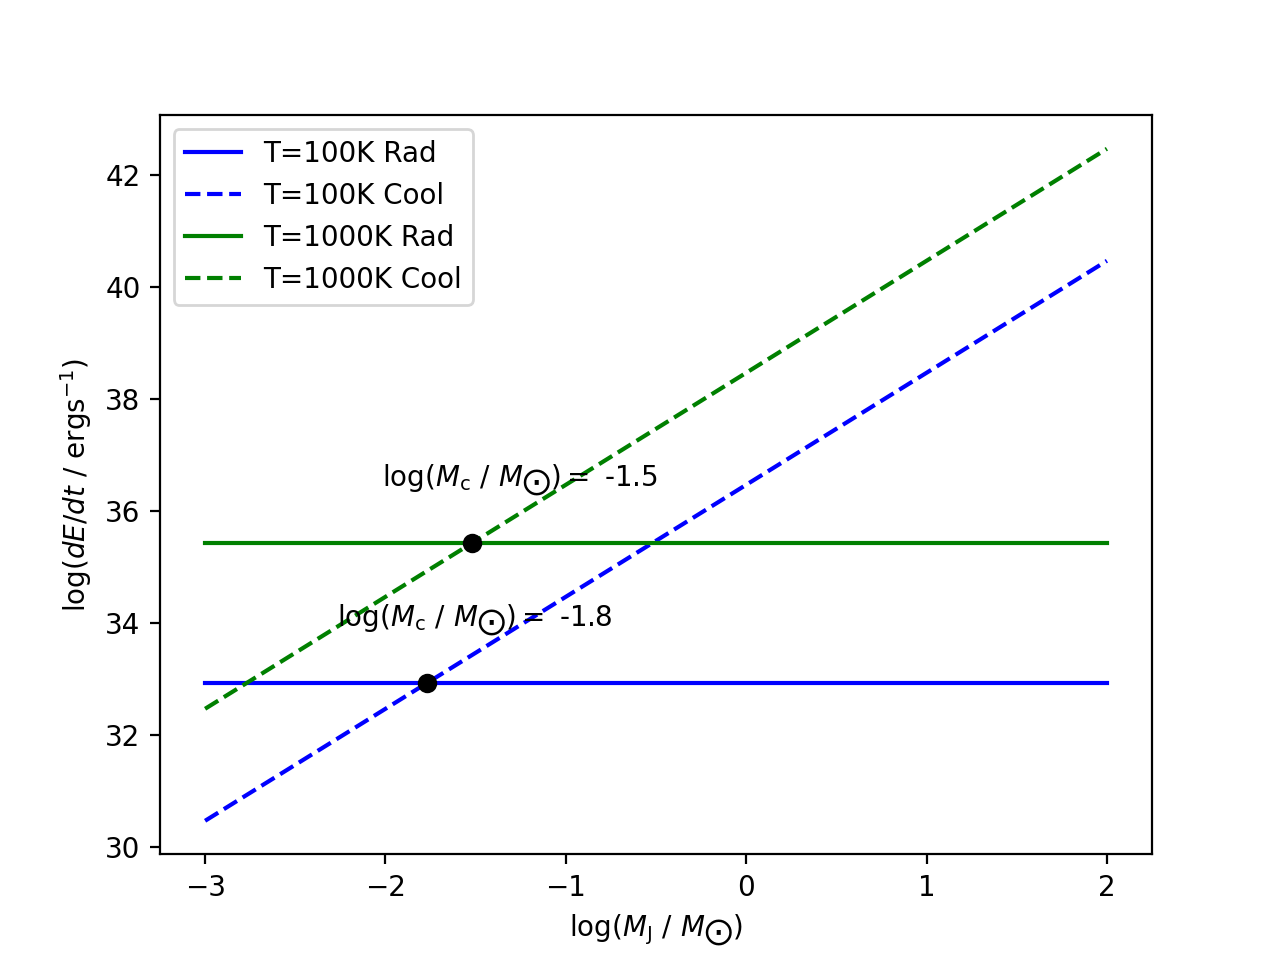
\includegraphics[width=10cm]{frag.png}
    % \caption{The relation}
\end{figure}

\subsection*{(f)}
Fragmentation stops at this point because if the Jeans Mass gets further smaller, 
the rate of radiation will be greater than the rate of cooling. When the rate of radiation 
is greater than the rate of cooling, cooling becomes uneffective and 
heat will be trapped, transforming the process from isothermal to adiabatic and 
increasing the Jeans Mass. With the Jeans Mass increased, the fragmentation stops.

\section*{\textbf{Exercise \uppercase\expandafter{\romannumeral3}.2  The Messier 80 globular cluster}}  
\subsection*{(a)}
The relatino between magnitude and flux is:
\begin{align*}
    m_1 - m_2 = -2.5 \log (F_1/F_2) \\
    F_1/F_2 = (L_1 / L_2) \cdot (d_2 / d_1)^2 
\end{align*}
We can rewrite the first equation as:
\begin{align*}
    \frac{L_1}{L_2} = 10^{\frac{m_1 - m_2}{-2.5}} (\frac{d_1}{d_2})^2
\end{align*}
For Messier 80, we have $m_1 = 7.87$; 
for Vega, we have $m_2 = 0.026$, $d_2 = 7.7 \text{pc}$ and $L_2 = 40 L_{\bigodot} $. 
Pluge in those concrete numbers and we have:
\begin{align*}
    \frac{L_{\text{M81}}}{L_{\bigodot}} &= A_1 (\frac{d}{\text{pc}})^2 \\
    A_1 &= 4.9 \times 10^{-4}
\end{align*}

\subsection*{(b)}
Assume that the stellar density follows an n = 5 polytrope with scaling parameter $R_s=\sqrt{3}\lambda_5$, and the 
solution for the $n=5$ polytrope is that:
\begin{align*}
    \phi_5 = (1 + \frac{R^2}{R_s^2})^{-1/2}
\end{align*}
where $\rho  = \rho_c \phi_5^5$. Therefore, the density for the polytrope is:
\begin{align*}
    \rho(r, \phi , z) = \rho_c (1 + \frac{r^2 + z^2}{R_s^2})^{-5/2}
\end{align*}
We define the stellar surface density at the distance $r$ from the center is $\Sigma(r)$, which 
satisfies:
\begin{align*}
    \Sigma(r) 2\pi r \d r &= \int \int \rho(r, \phi, z) r\d r \d \phi \d z \\
    \Sigma(r) &= \rho_c \int_{-\sqrt{R_s^2-r^2}}^{\sqrt{R_s^2-r^2}} (1 + \frac{r^2 + z^2}{R_s^2})^{-5/2} \d z \\
    \Sigma(r) &= 2\rho_c R_s \int_{a}^{1} (1+u^2)^{-5/2} \frac{u}{\sqrt{u^2 - a^2}} \d u
\end{align*}
where $a = \frac{R_c}{R_s}$ and $u = \sqrt{R_c^2 + z^2}$.
The stellar surface density at the distance $R_c$ is half of that $\rho_c R_s$ at the center, so we can solve the 
equation for $a$:
\begin{align*}
    &\int_{a}^{1}(1+u^2)^{-5/2} \frac{u}{\sqrt{u^2 - a^2}} \d u = 1/4 \\
    &a = 0.64
\end{align*}
that is $R_c=0.64R_s$.

\subsection*{(c)}
The mass-to-luminosity ratio (M/L) of globular clusters is higher than that of the Sun 
because globular clusters are composed of old stars that have low metallicity and are deficient in heavy elements. 
This means that they have fewer heavy elements than younger stars like the Sun. 
The M/L ratio is also affected by the presence of dark matter in globular clusters.

\subsection*{(d)}
Assuming the 1D velocity of stars in the M80 globular cluster obeys 1D Maxwell distribution:
\begin{align*}
    f(v_x)dv_x = (\frac{m}{2\pi kT})^{1/2} \exp(-\frac{m v_x^2}{2kT}) d v_x
\end{align*}
From an analogy of the gaussian distribution, we can see that the dispersion in the 1D velocity 
is related to the temperature of the globular cluster:
\begin{align*}
    \frac{kT}{m} = \sigma^2 \\
    kT = m \sigma^2
\end{align*}
where $m$ is the mean mass of the stars and $\sigma$ is the one dimensional velocity dispersion.
According to the Virial Theorem, we can derive the total mass of Messier:
\begin{align*}
    W + 2 U_{\text{int}} &= 0\\
    -\frac{3\pi}{32} \frac{GM^2}{R_s} + 2 \frac{3}{2} kT \frac{M}{m} &= 0 \\
    M = \frac{32}{\pi} & \frac{\sigma^2 R_s}{G}
\end{align*}
Therefore, the luminosity of Messier 80 can be written as:
\begin{align*}
    \frac{L_{\text{M81}}}{L_{\bigodot}} = 0.2 \frac{M}{M_{\bigodot}} = \frac{6.4}{\pi} \frac{\sigma^2 R_s}{G M_{\bigodot}} =  A_1 (\frac{d}{\text{pc}})^2
\end{align*}
And from the `core radius' we can have derive the relation between $R_s$ and $d$:
\begin{align*}
    R_s = \frac{1}{0.64} R_c = \frac{1}{0.64} d \Delta \theta
\end{align*}
where $\Delta \theta$ is the observed angular length of the core. Therefore:
\begin{align*}
    \frac{d}{\text{pc}} = \frac{10}{\pi} \frac{\sigma^2 R_s}{G M_{\bigodot}} \frac{\text{pc} \Delta \theta}{A_1} \approx 5.86 \times 10^3
\end{align*}
our distance to M80 is $d = 5.86 \text{kpc}$.

\section*{\textbf{Exercise \uppercase\expandafter{\romannumeral3}.3  The initial mass function (IMF)}}
\subsection*{(a)}
The number fraction of Broen Dwarfs $f(n)$ is:
\begin{align*}
    f(n) = \frac{\int_{0}^{0.075} \xi(m) \d m}{\int_{0}^{\infty } \xi(m) \d m} = 20.8\%
\end{align*}
The mass fraction of Broen Dwarfs $f(m)$ is:
\begin{align*}
    f(m) = \frac{\int_{0}^{0.075} m \xi(m) \d m}{\int_{0}^{\infty } m \xi(m) \d m} = 1.27\%
\end{align*}

\subsection*{(b)}
Seeing all stars out to a certain magnitude $m_0$ is the same as 
seeing all stars out to a certain flux $F_0$. Considering the critical situation, 
$L/d^2 \propto F_0$, and we can get $d \propto L^{1/2} \propto m^{\eta/2}$.

\subsection*{(c)}
We can see the stars on two condtions: they are within a certain distance  because we can only see out 
stars to a certain apparent magnitude; they are within their lifetime . 
Assume that all the stars are formed at a constant speed and are evenly distributed in the space.
Therefore, the number of stars $\d N$ of mass within $(m, m+\d m)$ that we can see is proportional to 
their lifetime $t_0$ and the largest distance we can see out to $d_0$:
\begin{align*}
    \d N \propto t_0 d_0^3 \xi(m) \d m \propto m^{1-\eta} m^{\frac{3\eta}{2}} m^{-2.35} \d m = m^{\frac{\eta}{2}-1.35} \d m
\end{align*}
When $\eta=3.5$, $\frac{\d N}{\d m} = m^{0.4}$, so most stars we see are massive.

\section*{\textbf{Exercise \uppercase\expandafter{\romannumeral3}.4 Toomre-Q and disk instability}}
\subsection*{(a)}
\begin{align*}
    E_{\text{therm}} &= kT \frac{M}{\mu m_u} = c_s^2 M = c_s^2 \Sigma \lambda^2 \\
    E_{\text{grav}} &= - \frac{G M^2}{\lambda} = - \frac{G (\Sigma \lambda^2)^2}{\lambda} = -G\Sigma^2 \lambda^3 \\
    E_{\text{rot}} &= \frac{1}{2} I \Omega^2 = \frac{1}{2} \Sigma \lambda^2 \lambda^2 \Omega^2 = \frac{1}{2} \Sigma \lambda^4 \Omega^2
\end{align*}
Pluge the above three relations into the inequation:
\begin{align*}
    \vert \frac{c_s^2 \Omega^2}{2 G^2 \Sigma^2} \vert < 1
\end{align*}
The above estimate results in $Q_T \sim \frac{c_s \Omega}{G \Sigma}$, barring a factor of unity.
% \begin{align*}
%     Q_T = \frac{c_s \Omega}{G \Sigma} \lesssim  1
% \end{align*}
\subsection*{(b)}
The disk becomes unstable when the Toomre-Q criterion is smaller than 1:
\begin{align*}
    Q_T = \frac{c_s \Omega}{\pi G \Sigma} < 1
\end{align*}
Considering $\Omega = \sqrt{\frac{GM_{\bigodot}}{r^3}}$, $c_s^2 = \frac{kT}{\mu m_u}$, 
we have:
\begin{align*}
    \sqrt{\frac{kT GM}{\mu m_u r^3}} < \pi G \Sigma
\end{align*}
Given that $T = 200 \ K (r/au)^{-1/2}$, $\Sigma = 2\times 10^3 \ \g \cm^{-2} (r/au)^{-1}$ and $\mu=2.3$, 
we can solve the inequation for $r$ and we get $r>139 \text{au}$. From $r=139 \text{au}$ and outward,
the disk is unstable.

\subsection*{(c)}
The mass associated with the critical wavelength $\lambda_c$ is:
\begin{align*}
    M_c \sim \lambda_c^2 \Sigma \sim \frac{c_s^4}{G^2\Sigma}
\end{align*}
Pluge in $c_s^2 = \frac{kT}{\mu m_u} = \frac{k}{\mu m_u} 200 \ K (r/au)^{-1/2}$ and $\Sigma = 2\times 10^3 \ \g \cm^{-2} (r/au)^{-1}$, 
we get the mass associated with the critical wavelength is $M_c \sim 3.1 M_J$.

\section*{\textbf{Exercise \uppercase\expandafter{\romannumeral3}.5 Radial drift of solids in disks}}
\subsection*{(a)}
Maybe $t_\text{stop}$ is called `stopping time' because after being dragged by the tha gas for $t_\text{stop}$, 
the relative velocity between the gas and the particles will become zero. The particles will stop spiraling inward. 

\subsection*{(b)}
Since the tangential velocities of the particles and gas are the same, the relative velocity is equal to 
the radial velocity of the small particles. According to the Impulse Theorem:
\begin{align*}
    F_\text{drag} t_\text{stop} &= m \Delta v \\
    \Delta g_\text{drag} t_\text{stop} &= v_r \\
    v_r \simeq -2\eta \Omega_k^2 r  t_\text{stop} &= -2\eta v_k \Omega_k t_\text{stop}
\end{align*}
when $\Omega_k t_\text{stop} << 1$, the approximation is resonable.

\subsection*{(c)}
The angular momentum of a Keplerian circular orbit is:
\begin{align*}
    l &= mv_k r = m\sqrt{GMr} \\
    \d l / \d r &= \frac{m}{2} \sqrt{\frac{GM}{r}}
\end{align*}
The torque induced by the gas is:
\begin{align*}
    T = F_\text{drag} r = \frac{m \Delta v}{t_\text{stop}} r = \frac{m \eta v_k}{t_\text{stop}} r
\end{align*}
Therefore, the radial velocity of the large particles is:
\begin{align*}
    T = \d l / \d t = \frac{\d l}{\d r} \frac{\d r}{\d t} \\
    \vert v_r \vert = \frac{\d r}{\d t} = T \frac{\d r}{\d l} = \frac{2\eta r}{t_\text{stop}}
\end{align*}
When the large particles lose angular momentum, they drift inward, so considering the radial direction as 
positive the radial velocity should be $v_r = - \frac{2\eta r}{t_\text{stop}}$.

\subsection*{(d)}
The combined expression of the radial velocity can be:
\begin{align*}
    v_r = (2\eta v_k \Omega_k t_\text{stop} - \frac{2\eta r}{t_\text{stop}})\exp(-\frac{m}{m_c}) + \frac{2\eta r}{t_\text{stop}}
\end{align*}
where $m$ is the mass of the particles and $m_c$ is the critical mass. When 
$m\rightarrow 0$, $v_r \rightarrow 2\eta v_k \Omega_k t_\text{stop}$, small particle case
; when $m\rightarrow +\infty$, $v_r \rightarrow \frac{2\eta r}{t_\text{stop}}$, large particle case.

\subsection*{(e)}
Because $\Omega t_\text{stop} = 1$, the particles are large and the radial velocity should be calculated as 
$v_r = \frac{2\eta r}{t_\text{stop}}$. Given $t_\text{stop} \Omega = 1$:
\begin{align*}
    v_r &= 2\eta r \Omega_k = 2\eta \sqrt{\frac{GM}{r}} \\
    t_\text{dritf} &= \frac{r}{v_r} = \frac{1}{2\eta} \sqrt{\frac{r^3}{GM}}.
\end{align*}
Radial drift timescales:
\begin{enumerate}
    \item[] 1 au: $t_\text{drift} = 8.0 \times 10^1 \ \text{yrs}$
    \item[] 10 au: $t_\text{drift} = 2.5 \times 10^3 \ \text{yrs}$ 
    \item[] 100 au: $t_\text{drift} = 8.0 \times 10^4 \ \text{yrs}$ 
\end{enumerate}

\section*{\textbf{Exercise \uppercase\expandafter{\romannumeral3}.6 Planet formation}}
\subsection*{(a)}
The relative motion between $M$ and $m$ is the radial velocity of $m$ caused by the eccentricity of m-bodies.
The radial velocity of the m-bodies can be estimated as the radial difference at the aphelion and the  perihelion 
divided by one half of the orbital period.
\begin{align*}
    v_r &\sim  \frac{2c}{T/2} = \frac{2ea}{T/2} \\
    \Omega_k &= \frac{2\pi}{T} \\
    v_r &\sim \frac{2ea}{\pi } \Omega_k
\end{align*}
The scale height of the m-bodies is $H \sim ai = ae/2$, so the number density of the m-bodies is:
\begin{align*}
    n \sim \frac{\Sigma_m}{H m}
\end{align*}
Assuming the collision cross section is $\sigma_m = \pi R^2$, the collision time can be written as:
\begin{align*}
    t_\text{coll} = \frac{1}{n\sigma_m \Delta v} \sim \frac{1}{n\sigma_m v_r} = \frac{m}{4\Sigma_m R^2 \Omega_k}
\end{align*}
The mass increasing rate for $M$ is:
\begin{align*}
    \frac{\d M}{\d t} = \frac{m}{t_\text{coll}} = 4 \Sigma_m R^2 \Omega_k
\end{align*}
Therefore, the growth timescale of the M-body is:
\begin{equation*}
    t_\text{growth} = \frac{M}{\d M/\d t} = \frac{\pi}{3} \frac{R \rho_\bullet }{\Sigma_m \Omega_k} \sim \frac{R \rho_\bullet }{\Sigma_m \Omega_k}
\end{equation*}

\subsection*{(b)}
\begin{enumerate}
    \item[] 0.1 au: $t_\text{growth} = 1.77 \times 10^5 \ \text{yrs}$
    \item[] 1 au: $t_\text{growth} = 5.61 \times 10^7 \ \text{yrs}$ 
    \item[] 10 au: $t_\text{growth} = 1.77 \times 10^{10} \ \text{yrs}$ 
\end{enumerate}
The timescales are too long to explain the solar system's planets. As we all know, 
the age of the Sun is about 4.6Gyr and the age of the Earth is about 4.5Gyr. 
The timescale for 10au is larger than the age of the solar system.
Besides, the typical survival time of the protoplanetary disk is about a few Myrs, but 
according to our calculation, it needs more than 10 Myrs to form an Earth-mass planet at 1au.

\subsection*{(c)}
If we consider gravitational focusing, then the collision cross section will become:
\begin{align*}
    \sigma_g = \pi R^2 (1+(\frac{v_\text{esc}}{\Delta v})^2) = \pi R^2 (1 + \frac{2GM}{R \Delta v^2}) \sim \pi R^2 (1 + \frac{2GM}{R v_r^2})
\end{align*}
The mass increasing rate for M-body will become:
\begin{align*}
    \frac{\d M}{\d t} &= 4 \Sigma_m R^2 \Omega_k (1 + \frac{2GM}{R v_r^2})
\end{align*}
This is a differential equation for M, and we seperate variables:
\begin{align*}
    \frac{\d M}{1 + \frac{2GM}{R v_r^2}} = 4 \Sigma_m R^2 \Omega_k \d t
\end{align*}
We integrate the above equation and notice that $M(t=0)=0$:
\begin{align*}
    t_\text{growth} = \frac{v_r^2}{8G\Sigma_m R \Omega_k} \ln (1+\frac{2GM}{R v_r^2}) 
\end{align*}
Growth timescales:
\begin{enumerate}
    \item[] 0.1 au: $t_\text{growth} = 3.13 \times 10^3 \ \text{yrs}$
    \item[] 1 au: $t_\text{growth} = 1.38 \times 10^5 \ \text{yrs}$ 
    \item[] 10 au: $t_\text{growth} = 5.59 \times 10^6 \ \text{yrs}$ 
\end{enumerate}

\end{document}
